\NeedsTeXFormat{LaTeX2e}
\documentclass[12pt,a4paper,oneside,openright]{article}
%\pagestyle{empty}
\usepackage[utf8]{vietnam}
\usepackage[useregional]{datetime2}

% \usepackage{indentfirst}
\usepackage{amsmath,amsfonts,amssymb,fancyhdr}
\usepackage{amsthm,amsxtra,latexsym, amscd}
\usepackage[top=3.5cm, bottom=3cm, left=3.5cm, right=2.0cm] {geometry}
\usepackage[unicode, hidelinks]{hyperref}
\usepackage{titlesec}
\usepackage{boxedminipage,fancybox}
\usepackage{graphicx}
\usepackage{floatrow}
\usepackage{lastpage}
\usepackage{enumerate}
\usepackage{color}
\usepackage{graphicx}
\usepackage{array}
\usepackage{tabularx}
\usepackage{multirow}
\usepackage{multicol}
\usepackage{rotating}
\usepackage{graphics}
\usepackage{geometry}
\usepackage{setspace}
\usepackage{epsfig}
\usepackage{tikz}
\usepackage{placeins}
\usepackage{appendix}
\usepackage{booktabs}
\usepackage{float}
\usepackage{biblatex}
\usepackage[flushleft]{threeparttable}
\titleformat*{\subsubsection}{\large\bfseries} %set font size subsubsection
\titleformat*{\paragraph}{\large\bfseries}
\graphicspath{{images/}}
% \bibliography{references/tham_khao.bib}
%\hoffset=-0.3truecm %
%\voffset=-2.5truecm %
%\textheight=26truecm %
%\textwidth=16truecm %
%\oddsidemargin 28pt \footskip 30pt
\font\tench=t5-lmb10 at18pt%
\titleformat{\chapter}[display]
{\normalfont\large\filcenter\bfseries}
{{{\chaptertitlename\,}\thechapter}} {1pc}{%\vspace{1pc}%
{\tench}\MakeUppercase}% Dinh nghia lai ten chuong
%{\tench}}%\MakeUppercase}% Dinh nghia lai ten chuong
%\renewcommand{\theenumi}{\textbf{\arabic{enumi}}}%Danh lai so thu tu
%\renewcommand{\labelenumi}{\theenumi )}%Danh lai so thu tu
\renewcommand{\theequation}{\thechapter.\arabic{equation}}% Danh lai so cong thuc toan
\font\tieude=t5-lmb10 at 14pt
 \pagestyle{fancy}
\renewcommand\headrulewidth{0 pt}
 \lhead{ }
 \chead{\thepage }
 \rhead{  }
\lfoot{ }
\cfoot{ }
\rfoot{ }
\numberwithin{subsection}{section}
%------------------------------------------------------------
\theoremstyle{definition}
%\swapnumbers
%{\theorembodyfont{\rmfamily}
\theoremstyle{plain}
\newtheorem{theorem}{Định lý}[section]
\newtheorem{dl}[theorem]{Định lý}
\newtheorem{hq}[theorem]{Hệ quđả}
\newtheorem{corollary}[theorem]{Hệ quả}
\newtheorem{problem}{Bài toán}
\newtheorem{main}{Định lý cơ bản}
\newtheorem{bd}[theorem]{Bổ đề}
\newtheorem{lemma}[theorem]{Bổ đề}
\newtheorem{md}[theorem]{Mệnh đề}
\newtheorem{proposition}[theorem]{Mệnh đề}
\theoremstyle{definition}
\newtheorem{dn}[theorem]{Định nghĩa}
\newtheorem{definition}[theorem]{Định nghĩa}
\theoremstyle{definition}
\theoremstyle{remark}
\theoremstyle{definition}
\newtheorem{note}[theorem]{\bf Chú ý}
\newtheorem{vd}[theorem]{\bf Ví dụ}
\newtheorem{example}[theorem]{Ví dụ}
\newtheorem{nx}[theorem]{\bf Nhận xét}
\newtheorem{remark}[theorem]{Nhận xét}
\newtheoremstyle{vd}% name
  {3pt}%      Space above
  {3pt}%      Space below
  {}%         Body font
  {}%         Indent amount (empty = no indent, \parindent = para indent)
  {\bfseries}% Thm head font
  {.}%        Punctuation after thm head
  {.5em}%     Space after thm head: " " = normal interword space;
        %       \newline = linebreak
  {}%

%-----------------------------------------------------------------------

%\includeonly{bia1}
\usepackage{cleveref}
\crefformat{figure}{hình~#2#1#3}

\begin{document}
% \cref{fg:adc}
\font\chuong=t5-lmb10 at12pt%
 \def\chaptername{\chuong CHƯƠNG}
\fontsize{14pt}{14pt}\selectfont% Chon cỡ font

\newcommand{\set}[1]{\mathbb{#1}}
\providecommand{\keywords}[1]{\textbf{\textit{Từ khóa---}} #1}


\begin{figure}[h!]
  \caption{Quá trình giải bài toán Machine learning}
  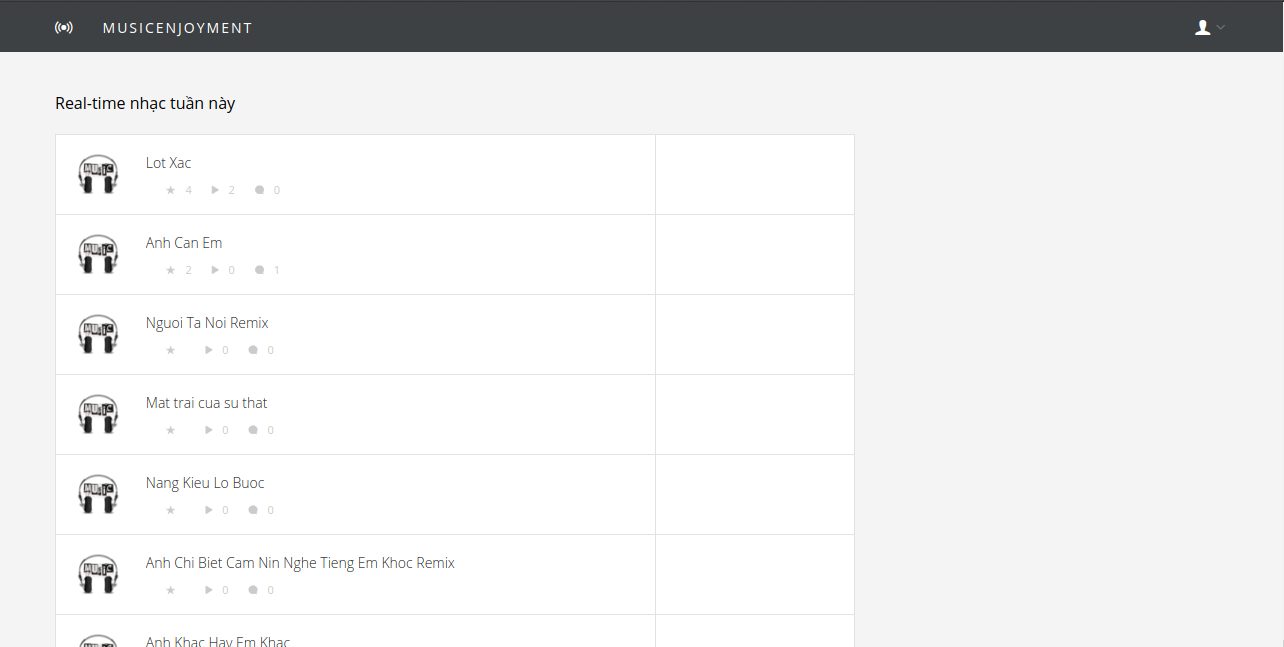
\includegraphics[width=\textwidth]{bxh.png}
  \label{bxh}
\end{figure}


\begin{figure}[h!]
  \caption{Quá trình giải bài toán Machine learning}
  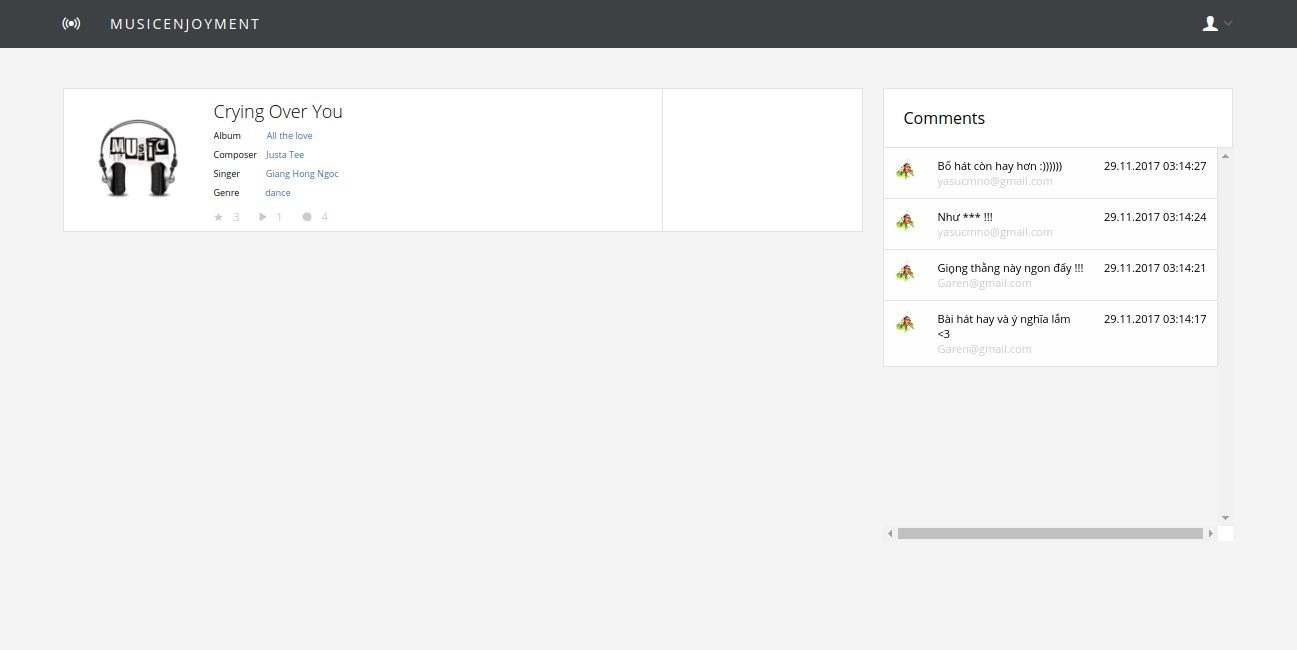
\includegraphics[width=\textwidth]{nhac.png}
  \label{nhac}
\end{figure}


\begin{figure}[h!]
  \caption{Quá trình giải bài toán Machine learning}
  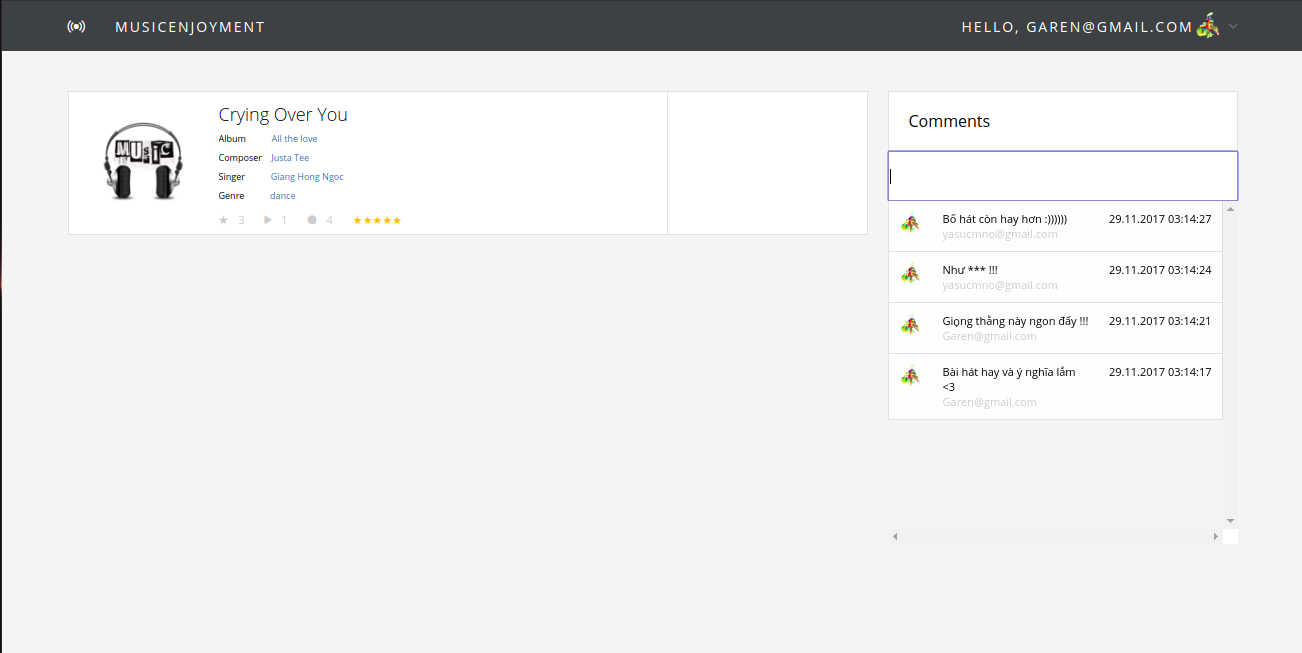
\includegraphics[width=\textwidth]{nhac-login.png}
  \label{fg:nhac-login}
\end{figure}


\begin{figure}[h!]
  \caption{Quá trình giải bài toán Machine learning}
  \includegraphics[width=\textwidth]{supervised.png}
  \label{fg:supervised}
\end{figure}


\begin{figure}[h!]
  \caption{Quá trình giải bài toán Machine learning}
  \includegraphics[width=\textwidth]{supervised.png}
  \label{fg:supervised}
\end{figure}


\begin{figure}[h!]
  \caption{Quá trình giải bài toán Machine learning}
  \includegraphics[width=\textwidth]{supervised.png}
  \label{fg:supervised}
\end{figure}


\begin{figure}[h!]
  \caption{Quá trình giải bài toán Machine learning}
  \includegraphics[width=\textwidth]{supervised.png}
  \label{fg:supervised}
\end{figure}


\end{document}

%%21:16:49 1/9/2012Last Modification of contents